\chapter{Introduction to Buses and Mastering}
\label{chap:bus-mastering}

A bus is where several tracks meet and get processed together; mastering is the final bus pass and delivery check before the song leaves the building. Yeban has no separate mastering suite. It has three real entry points: auxiliary return tracks (\texttt{AuxReturn}), the master bus (\texttt{Master}) with its fader and insert chain, and the export dialog with its bus limiter, format settings and post-export measurement line. Loudness targets, true-peak ceilings and loudness normalization exist only on the CLI/MCP path; the GUI has no fields for them, and this chapter does not pretend otherwise.

\section{Signal flow from tracks to file}

The bus path can be reduced to one sentence: track device chain $\rightarrow$ track fader/pan $\rightarrow$ send edge $\rightarrow$ auxiliary return $\rightarrow$ master sum $\rightarrow$ master fader $\rightarrow$ master insert chain $\rightarrow$ export limiter (optional) $\rightarrow$ quantization/dither $\rightarrow$ WAV.

\begin{center}
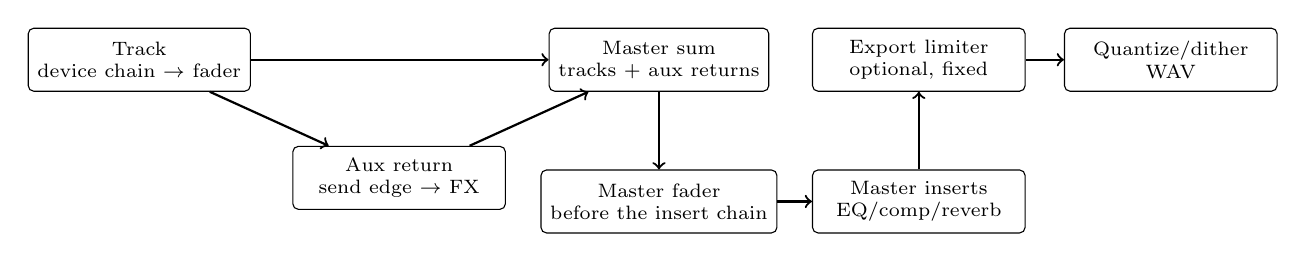
\begin{tikzpicture}[
  box/.style={draw, rounded corners=2pt, minimum width=27mm, minimum height=8mm, align=center, font=\scriptsize},
  arrow/.style={->, thick}
]
  \node[box] (trk) at (0,0) {Track\\device chain $\rightarrow$ fader};
  \node[box] (aux) at (3.3,-1.5) {Aux return\\send edge $\rightarrow$ FX};
  \node[box] (sum) at (6.6,0) {Master sum\\tracks + aux returns};
  \node[box] (fader) at (6.6,-1.8) {Master fader\\before the insert chain};
  \node[box] (ins) at (9.9,-1.8) {Master inserts\\EQ/comp/reverb};
  \node[box] (lim) at (9.9,0) {Export limiter\\optional, fixed};
  \node[box] (out) at (13.1,0) {Quantize/dither\\WAV};
  \draw[arrow] (trk) -- (aux);
  \draw[arrow] (trk) -- (sum);
  \draw[arrow] (aux) -- (sum);
  \draw[arrow] (sum) -- (fader);
  \draw[arrow] (fader) -- (ins);
  \draw[arrow] (ins) -- (lim);
  \draw[arrow] (lim) -- (out);
\end{tikzpicture}
\end{center}

The master fader sits \textbf{before} the insert chain, not after it. Push the fader up and the level entering EQ, compression and reverb rises with it; the export limiter is the last stage after the inserts. Do not use the master fader to compensate a limiter, and do not treat it as mastering gain: the fader changes the drive into the insert chain, while the limiter changes the final ceiling.

\section{Auxiliary returns and sends}

An auxiliary return track has kind \texttt{AuxReturn}; it exists for summing and shared processing, not for hosting an instrument. There are two creation entries:

\begin{itemize}
  \item the track menu item ``+ New auxiliary bus track'';
  \item the device rack's ``+ Aux return'' button in the send area.
\end{itemize}

Once it exists, open a display track's device rack, click ``New send'', and choose that auxiliary return as the destination. A send edge carries one gain field, \texttt{gain\_db}; there is no pre/post switch. The UI has no ``send point before/after fader'' choice, so do not assume another DAW's pre/post convention.

\screenshot{bus-aux-send}{Device rack send area showing a send edge to an auxiliary return, with the aux effect chain and send gain visible}

Auxiliary returns are for processing shared by several tracks:

\begin{table}[htbp]
\centering
\small
\begin{tabular}{@{}p{0.22\linewidth}p{0.30\linewidth}p{0.38\linewidth}@{}}
\hline
Use & Where & Reason \\
\hline
Shared reverb & Reverb on the aux return; level via the send-edge gain & Several tracks feed one reverb and share one tail; do not insert an identical reverb on every track \\
Shared delay & Delay on the aux return & One delay time/feedback for alignment \\
Group compression & Several tracks into one aux return, then to master & Compress only that group, not the whole song; the aux fader still rides the group \\
\hline
\end{tabular}
\caption{Common uses of auxiliary returns}
\label{tab:aux-return-uses}
\end{table}

For a shared reverb, set the reverb device to mostly wet and little dry; the dry signal still travels directly from the source track to the master. Otherwise the same dry signal appears again in the aux return and becomes double dry. The send-edge gain is absolute dB, not a percentage; lowering it lowers the level into the reverb but does not change the source track's direct path.

\section{The master bus chain}

The master bus track has kind \texttt{Master}. Select it and press \texttt{F9} to open the device rack and see its insert chain; press \texttt{X} or \texttt{F8} to open the mixer console and see the master fader, meters and channel strip.

What the master bus can do:

\begin{table}[htbp]
\centering
\small
\begin{tabular}{@{}p{0.22\linewidth}p{0.34\linewidth}p{0.34\linewidth}@{}}
\hline
Stage & Entry point & Do not use it for \\
\hline
Summing & the routing graph feeds every track/aux return into \texttt{Master} & fixing one track's frequency response or dynamics \\
Fader & master fader in the mixer console (F8/X) & replacing a limiter or loudness normalization \\
Insert chain & EQ, Compressor, Reverb, Delay, Limiter, etc.\ on the master device rack & stacking a long ``mastering preset''; every device needs a stated reason \\
Export limiter & the bus limiter switch in the export dialog & an adjustable mastering limiter; it is fixed and per-export \\
\hline
\end{tabular}
\caption{What each master-bus stage is for, and what it is not for}
\label{tab:master-stages}
\end{table}

\screenshot{master-bus-chain}{Mixer console with the master bus selected, showing the master fader, meters and the master insert chain in the device rack}

Bus processing starts with ``fix the source first, then fix the bus''. A single track that is too bright, too loud or too bass-heavy should be fixed on that track's EQ/compressor/fader; the master should only handle problems shared by every track: overall dynamics, overall tonal balance, overall space. Pulling 3 dB of low end on the master is often paying for excess low end on several tracks, and the fix will not transfer to the next arrangement.

\subsection{Three common bus stages}

\begin{enumerate}
  \item \textbf{Master EQ}: small corrections only. Use the channel-strip low cut to remove inaudible/DC-adjacent energy below 20--30 Hz; move the mid/high region by 1--2 dB only when the whole mix is too bright or too dark. Do not use the master to sweep for a single track's problem.
  \item \textbf{Master compression}: use Compressor as glue, usually only 1--3 dB of gain reduction; start around 2:1, with an attack that does not grab transients and a release that does not pump. The compressor is in the insert chain and the fader is before it, so pushing the fader changes the compressor input; set the fader first, then the threshold.
  \item \textbf{Master limiting}: the Limiter device has threshold, ceiling, release, lookahead and a true-peak switch; the export dialog's bus limiter is a different fixed switch. Do not leave both on without knowing it, or you get two limiting stages and the second one is not adjustable.
\end{enumerate}

\subsection{Two limiters are not the same limiter}

\begin{table}[htbp]
\centering
\small
\begin{tabular}{@{}p{0.18\linewidth}p{0.27\linewidth}p{0.27\linewidth}p{0.20\linewidth}@{}}
\hline
 & Device-chain Limiter & Export-dialog limiter & Loudness normalization \\
\hline
Position & inside the master insert chain & after the master fader/automation, before quantization & after rendering, before quantization \\
Parameters & threshold/ceiling/release/lookahead/true peak & fixed 0.9 threshold, 0.95 ceiling, 33-frame lookahead, true-peak detection off & target LUFS + true-peak ceiling (CLI/MCP) \\
Default & exists only when inserted & off & no target, no action \\
Adjustable & device parameters & on/off only & target and ceiling \\
Stored in project & yes (device chain) & no (per-export modifier) & no (per-export modifier) \\
\hline
\end{tabular}
\caption{Device-chain limiter, export limiter and loudness normalization are different things}
\label{tab:limiters}
\end{table}

The export-dialog limiter has a 33-frame lookahead; the export path compensates those 33 frames, so output length and timeline do not change. Its ceiling of linear 0.95 is about $-0.45$ dBFS and its threshold of 0.9 is about $-0.92$ dBFS. It does not do true-peak oversampling, so it cannot guarantee ``true peak below $-1$ dBTP''; for that guarantee, read the post-export measurement or use the CLI/MCP loudness normalization/true-peak ceiling.

\section{Loudness readings: UI and export are not the same}

Yeban's UI shows the letters ``LUFS'', but the live readings and the export readings must be kept apart:

\begin{table}[htbp]
\centering
\small
\begin{tabular}{@{}p{0.24\linewidth}p{0.30\linewidth}p{0.38\linewidth}@{}}
\hline
Reading & Source & Can it be a delivery reference? \\
\hline
Mixer master LUFS & master smoothed RMS minus 0.691 dB & only a rough level guide; not BS.1770 gated integrated loudness, so do not report ``the song is $-14$ LUFS'' from it \\
Control-room short-term LUFS & same master reading & same; it has no 3 s short-term window and no gating \\
Control-room integrated LUFS & no runtime update in the current build; only the UI default string & not a reading; do not screenshot it as evidence \\
Control-room dBTP & no runtime update; only the UI default string & not a reading; true peak exists only in the post-export measurement \\
Post-export measurement & 16$\times$ true peak, gated integrated LUFS, LRA & the only usable delivery reading; unmeasurable values are printed as ``not measured'' \\
\hline
\end{tabular}
\caption{LUFS in the UI versus the post-export measurement}
\label{tab:loudness-readings}
\end{table}

This is not nitpicking about names. The master reading is ``smoothed RMS minus 0.691 dB'', without BS.1770 K-weighting, gating, or the 400 ms/3 s windows. It can tell you roughly how loud the program is, but it cannot prove ``this song reaches $-14$ LUFS''. The control room's integrated LUFS and dBTP fields have no runtime writer in the current build; their default strings are placeholders. To get a delivery reading, export once and read the measurement line.

\screenshot{export-wav-dialog}{WAV export dialog: sample rate, bit depth, duration, bus limiter switch, and the post-export measurement line}

The three numbers in the post-export line are:

\begin{itemize}
  \item \textbf{True peak}: a dBFS reading from 16$\times$ oversampling; 0 is full scale, positive values are over.
  \item \textbf{Integrated loudness}: BS.1770-4 gated integrated LUFS; programs shorter than 400 ms, or entirely below the absolute gate, show ``not measured''.
  \item \textbf{LRA}: P95$-$P10 of the 3 s short-term histogram with a $-20$ LU relative gate; shorter than 3 s, or no short-term value above the gate, shows ``not measured''.
\end{itemize}

\section{Export options and loudness targets}

The WAV export dialog has five real controls:

\begin{table}[htbp]
\centering
\small
\begin{tabular}{@{}p{0.16\linewidth}p{0.24\linewidth}p{0.50\linewidth}@{}}
\hline
Control & Default & Semantics \\
\hline
Output path & none & browse or type; filling the path does not export \\
Sample rate & \texttt{auto} & follows the project; it does not display the project rate, so do not read \texttt{auto} as a fixed 48 kHz \\
Bit depth & \texttt{24} & 16/24-bit integers use TPDF dither; 32f floats pass through without dither \\
Seconds & audible project end & seeded when the dialog opens; clearing it falls back to the 8 s default, not the whole song. Check long tails and silent tails yourself \\
Bus limiter & off & a per-export boolean; fixed parameters; not stored in the project, not undoable \\
\hline
\end{tabular}
\caption{The real controls in the WAV export dialog}
\label{tab:export-options}
\end{table}

The GUI has \textbf{no} controls for: loudness target (LUFS), true-peak ceiling, peak normalization, dither mode, noise shaping or mastering clipper. They are not in the export dialog; do not write a GUI procedure that claims ``set $-14$ LUFS here''.

Only the CLI/MCP path has loudness normalization:

\begin{table}[htbp]
\centering
\small
\begin{tabular}{@{}p{0.22\linewidth}p{0.20\linewidth}p{0.20\linewidth}p{0.30\linewidth}@{}}
\hline
Preset & Target LUFS & True-peak ceiling & Entry \\
\hline
Streaming & $-14$ & $-1$ dBTP & CLI/MCP; not the GUI \\
EBU R128 & $-23$ & $-1$ dBTP & CLI/MCP; not the GUI \\
\hline
\end{tabular}
\caption{Built-in loudness presets; the numbers are product choices, not a normative mandate}
\label{tab:loudness-presets}
\end{table}

MCP rendering's \texttt{targetLufs} accepts $[-70,0]$; when supplied, it applies gain to reach the target, with a true-peak ceiling of $-1.0$ dBTP as the binding limit. It re-measures with a $\pm0.5$ LU tolerance and fails loudly with \texttt{RENDER\_FAILED} if the target is missed; it never silently ships an off-target file. The CLI also has \texttt{--true-peak-ceiling} for setting the ceiling independently. Loudness normalization is available only at 44.1/48/88.2/96 kHz; other sample rates fail instead of silently falling back to 48 kHz coefficients.

For a range export the target is measured on the \textbf{exported slice}, not the whole song. A stem target and a full-song target are not the same thing; do not apply the full song's $-14$ to an eight-second stem and ask why the reading differs.

\section{Pre-export checklist}

\begin{enumerate}
  \item \textbf{Check the sources}: is any single track too bright, too loud or too bass-heavy? Fix it on the track, not on the master.
  \item \textbf{Master fader}: make sure it is not pushed far past 0 dB just to ``sound louder''; it sits before the insert chain, so it changes the compressor/limiter input.
  \item \textbf{Insert chain}: confirm bypass states and parameters one device at a time; do not leave both the device-chain Limiter and the export limiter on without knowing it.
  \item \textbf{Export once with the limiter off}: read the post-export true peak, integrated LUFS and LRA as the unrestricted baseline.
  \item \textbf{Clipping warning}: if ``master clipped N samples, reduce by X dB'' appears, follow the suggestion on the master or the loudest source; do not ignore it and ship anyway.
  \item \textbf{Targets}: when a target is required, use the CLI/MCP \texttt{targetLufs}/\texttt{--loudness-target}, not the GUI; confirm the sample rate is supported.
  \item \textbf{Format}: 24-bit integer (TPDF) is the common delivery choice; use 32f when downstream processing continues; use 16-bit only when the downstream explicitly asks. Keep the project sample rate unless there is a delivery reason to change it.
  \item \textbf{Duration}: confirm the seconds field is not the 8 s default; include the outro, silent tail and fade.
  \item \textbf{Final listen}: use the F4 control room for MONO/SIDE checks; these switches do not affect export, so do not judge export level with MONO on.
\end{enumerate}

\begin{table}[htbp]
\centering
\small
\begin{tabular}{@{}p{0.28\linewidth}p{0.62\linewidth}@{}}
\hline
Check & Pass condition \\
\hline
Master clipping & post-export true peak is within the target ceiling; if a clipping warning appears, reduce the source or the master first \\
Loudness & within $\pm0.5$ LU when a target is set; without a target, record the measurement and do not claim compliance \\
Format & sample rate matches delivery; bit depth matches downstream; integer depths are dithered \\
Duration & covers the whole song, including the outro, not the 8 s fallback \\
Monitoring & no must-keep part disappears in MONO; no centred dry signal dominates SIDE \\
\hline
\end{tabular}
\caption{Pre-export checklist}
\label{tab:export-checklist}
\end{table}

\section{Not yet provided, and boundaries}

\begin{table}[htbp]
\centering
\small
\begin{tabular}{@{}p{0.34\linewidth}p{0.54\linewidth}@{}}
\hline
Request & Current state in Yeban \\
\hline
A separate mastering suite & none; only the master insert chain and export options \\
Multiband compression/dynamic-EQ mastering chain & no separate mastering multiband compressor; the channel strip has EQ/compression stages, but that is not a mastering suite \\
GUI loudness target/true-peak ceiling & none; CLI/MCP only \\
Live integrated LUFS/true peak/LRA in the UI & none; control-room integrated and dBTP fields have no runtime writer, and the master LUFS is RMS$-$0.691 \\
Automatic loudness matching/reference level alignment & none; the reference track is for A/B only, with no automatic level match \\
Send pre/post switch & none; a routing edge has gain only \\
Dither mode/noise shaping & none; integer depths use fixed TPDF, 32f passes through \\
An absolute ``never clips'' true-peak guarantee & none; 16$\times$ still has inherent under-read, so the reading is not a mathematical guarantee \\
Storing export-limiter settings in the project & none; it is a per-export boolean \\
\hline
\end{tabular}
\caption{Current boundaries of buses and mastering}
\label{tab:mastering-gaps}
\end{table}

\section{Help-topic mapping}

\begin{table}[htbp]
\centering
\small
\begin{tabular}{@{}p{0.34\linewidth}p{0.52\linewidth}@{}}
\hline
Section & In-app help anchor \\
\hline
Signal flow from tracks to file & \texttt{master-signal-flow} \\
Auxiliary returns and sends & \texttt{aux-return-sends} \\
The master bus chain & \texttt{master-bus-chain} \\
Two limiters are not the same & \texttt{master-limiters} \\
Loudness readings: UI and export & \texttt{loudness-readings} \\
Export options and loudness targets & \texttt{export-options-loudness} \\
Pre-export checklist & \texttt{export-checklist} \\
Current boundaries & \texttt{mastering-gaps} \\
\hline
\end{tabular}
\caption{Chapter 9 help-topic mapping}
\label{tab:mastering-help-map}
\end{table}
